% JuliaCon proceedings template
\documentclass{juliacon}
\setcounter{page}{1}

\lstset{literate=
{─}{{\ucc{$--$}}}{1}
{±}{{\ucc{$\pm$}}}{1}
}

\begin{document}

% **************GENERATED FILE, DO NOT EDIT**************
\title{JuliaDB: addressing the two-language problem in analytical databases}

\author[1, 2]{Shashi Gowda}
\author[2]{Jeff Bezanson}
\author[2]{Josh Day}
\author[2]{Stefan Karpinski}
\author[2]{Viral B. Shah}
\author[3]{Pietro Vertechi}
\author[1]{Alan Edelman}
\affil[1]{Massachusetts Institute of Technology}
\affil[2]{Julia Computing Inc.}
\affil[3]{Champalimaud Centre for the Unknown}

\keywords{Julia, Databases, Analytics, Generic Programming}



\maketitle

\begin{abstract}
We describe how the two-language problem manifests in the world of analytical databases. A system with this problem takes at least two languages to implement: a low-level statically compiled language such as C or C++ to implement the performance-sensitive operations, and a high-level dynamic scripting language such as Python or R to implement the user-facing API. This dichotomy usually exists because the latter language cannot compile to efficient machine code like the former, and the former does not have the ease-of-use as the latter. We present JuliaDB, a distributed database for analytical workloads that is built solely in Julia and does not have this and other resulting problems. JuliaDB is designed to allow seamless use of user-defined Julia functions and data types. Julia's just-in-time compilation welds code from across Julia's package ecosystem as well as user code to generate efficient machine code allowing for high-performance data science in a coherent environment. We show a case study involving the use of a custom numeric type. Our benchmark shows that the system can perform on-par with or betters that of pandas and tidyverse in the cases we tested.

\headingtable

\end{abstract}

\section{Introduction}

In~\cite{bezanson2017julia}, we describe the motivation behind Julia and how it was designed to address the two language problem: 
\begin{quote}
As long as the developers’ language is harder to
grasp than the users’ language, numerical computing will always be hindered. This is an essential part of the design philosophy of Julia: all basic functionality must be possible to implement in Julia—never force the programmer to resort to using C or Fortran.
\end{quote}

Modern data science workflows fall into two categories both of which show symptoms of the two language problem, the categories are:

\begin{enumerate}
\item Data is stored in traditional transaction-oriented databases (e.g. as Postgres and MySQL), queried with SQL, and analysed in high-level languages such as Python or R. This pairing suffers from two limitations: a) Most dialects of SQL, restrict custom data types and user defined functions, and b) The database server deals with on-disk data in a separate memory space from that of the analytics language making it an awkward combination for data science tasks.

\item Systems such as Pandas~\cite{mckinney-proc-scipy-2010} for Python and dplyr~\cite{dplyr} for R that provide a data storage and retrieval layer that is native to the host language. While they bring
the data into the memory space of the analytics language, they still
have some disadvantages: a) users must use vectorized database operations for performance since iterating over items in a loop can be expensive, and b) the need for vectorized operations to be 
implemented in C++, making it difficult to work with user defined data and functions. 
\end{enumerate}

Spark~\cite{spark} when used with Scala addresses many of the fundamental issues described above. However, Scala has been known to have performance concerns due to the design choices in the language~\cite{scalaslow}. In addition, users often use Spark through PySpark~\cite{pyspark} or SparkR~\cite{sparkr}, to gain the benefits of dynamically typed analytical languages. This brings us back to the two language problem.

We address the above mentioned two language problem in analytical databases with Julia~\cite{bezanson2017julia}. Its dynamic typing encourages exploratory and incremental programming. At the same time, users and database implementors have fine grained control over the memory layout of data. Struct types can be stored inline within arrays allowing efficient storage of user-defined
types. The just-in-time compiler can optimize data base operations and user defined functions as one system. Code from various packages written without the database in mind
can be used without performance penalties. In general, Julia finds the sweet-spot between dynamic
hassle-free languages such as Python and R helping the data scientist,
and efficient manually-memory-managed languages such as C or C++ helping
the database implementer greatly.



\section{Design of JuliaDB}

In the following subsection we describe the design of JuliaDB which empowers performance and interoperability.

\subsection{Columnar memory layout}
The basic datastructure in JuliaDB is the table.

\begin{lstlisting}[language=Julia]
lotr = table((name=StringArray(["Frodo", "Samwise", "Bilbo",
                                "Aragorn", "Boromir", "Gimli",
                                "Elrond", "Legolas"]),
             race=PooledArray(["Hobbit", "Hobbit", "Hobbit",
                               "Human", "Human", "Dwarf",
                               "Elf", "Elf"]),
             age=[33, 61, 111, 87, 41, 139, 6000, 2931]));

collect(lotr)

#=
8-element Array{NamedTuple{(:name, :race, :age),
                Tuple{String,String,Int64}},1}:
 (name = "Frodo", race = "Hobbit", age = 33)  
 (name = "Samwise", race = "Hobbit", age = 61)
 (name = "Bilbo", race = "Hobbit", age = 111) 
 (name = "Aragorn", race = "Human", age = 87) 
 (name = "Boromir", race = "Human", age = 41) 
 (name = "Gimli", race = "Dwarf", age = 139)  
 (name = "Elrond", race = "Elf", age = 6000)  
 (name = "Legolas", race = "Elf", age = 2931) 
=#
\end{lstlisting}
Listing 1. \emph{A table stores a named tuple of columns, but produces named tuple rows when iterated.}\\

Listing 1 shows a table constructed from a named tuple of column vectors. Although a table stores data as a named tuple of columns, it acts as an iterator of rows. Rows are tuples or named tuples of items.

The columns can be accessed using the \texttt{columns} function (e.g. \texttt{rows(lotr)} returns a named tuple of column vectors provided to \texttt{table} during construction) while the rows can be accessed as an array of tuples using the \texttt{rows} function rows is a struct of arrays view into the columnar storage, unlike \texttt{table} which returns a JuliaDB table, \texttt{rows} returns a legitimate Julia array.

Tables support \texttt{map}, \texttt{reduce}, \texttt{groupreduce}, \texttt{groupby} and \texttt{join} operations.

Listing 1 also illustrates use of \texttt{StringArray} and \texttt{PooledArray} array types as columns. These special array types enable efficient packing of String and categorical data respectively.


\begin{figure*}[t]
\centerline{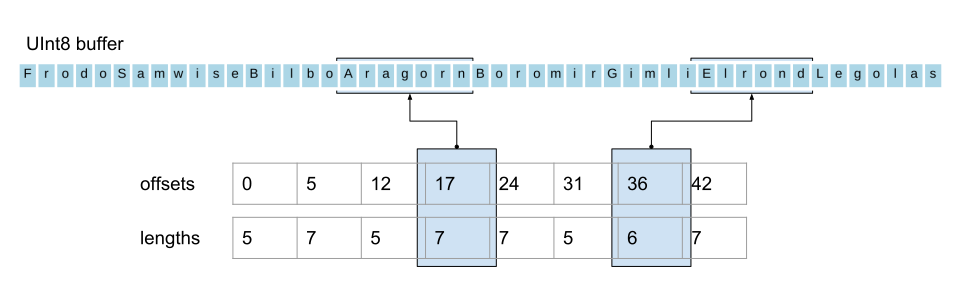
\includegraphics[width=11cm]{stringarray.png}}
\caption{StringArray layout.}
  \label{fig:stringarray}
\end{figure*}

A \texttt{StringArray}'s memory layout is show in in Figure \ref{fig:stringarray}. The contents of strings (unicode character codes) are packed into a buffer of 8-bit unsigend integers. \texttt{StringArray} also stores the lengths of each string and the index (offset) at which each of them starts. Although it would suffice to store just the length of each string, storing offset also allows us to implement efficient mutation operations. Setting an element of the array appends the new string to the end of the buffer and replaces the length and offset with the corresponding new length and offsets for that item. Operations such as \texttt{sort!} and \texttt{permute!} (in place permutation of items) can simply modify the length and offset arrays and leave the buffer unmodified. Wherever suitable, in code internal to JuliaDB, we create \texttt{WeakRefString} instead of creating String objects when we index into a \texttt{StringArray}, this greatly reduces GC-load when dealing with string columns in operations such as groupby and join.

A \texttt{PooledArray}'s memory layout is shown in Figure \ref{fig:pooledarray}. It is useful in compressing data with low number of unique items as compared to the total number of items. PooledArrays stores a dictionary mapping each unique item to a \texttt{ref} integer, and then an array of refs which tells which unique element appears in what position in the uncompressed array.

\subsection{Sort-based indexing}

We implement groupby and join by traversing tables in the key-order. We use counting sort wherever possible (e.g. integer columns, PooledArrays) to do a small amount of initial work on the order of $O(k \log k)$ where $k$ is the number of unique values and then achieve a sorted permutation in $O n$ time where $n$ is the number of rows. In most systems where the implementation is done in C++, the ordering routines are restricted to a handful of primitive data types. In our system any user defined data type with an \texttt{isless} method to compare two items can take part in the sorting.

\textbf{Indexing: }For speeding up table operations, you can tell
JuliaDB to keep the rows of a table sorted by some of its fields.
These fields are called primary key fields. The primary key fields
can be of any data type which has an \texttt{isless} method associated
with it to compare two values. This includes but is not limited to
numbers, strings, symbols, dates, time periods, currencies, quantities
of comparable physical units (e.g. inch, mm).

\subsection{Distributed compute}

A distributed table is a distributed analogue of the one described
above. It is stored as many tables across multiple Julia processes,
\texttt{columns} returns a tuple of \emph{distributed arrays} and
\texttt{rows} returns a distributed array of tuples! The distributed
arrays implementation has the usual array operations (map, reduce,
hcat, vcat) defined on it in a distributed manner. Constructing a
table with one or more distributed columns using the table constructor
results in a distributed table. We use the word ``table'' from now on to refer interchangeably to both types of tables, unless
noted otherwise.

\section{Case study: manipulating measurements}
\label{sec:measurements}

We take up a prototypical illustration of the power of JuliaDB by using a custom number type, namely the Measurement type, in a database.

Measurements.jl implements the ± operator which represents an observation with some uncertainty associated with it. Numeric operations on measuements propagate the uncertainty as prescribed by linear error propagation theory: For a function application $G(a,b,c...)$ where arguments are measurements $a=\overline{a} \pm \sigma_{a}, b=\overline{b} \pm \sigma_{b}, c=\overline{c} \pm \sigma_{c}$ the error of the output is found using the relationship: 

$$\begin{equation}
  \begin{align}
    \sigma_G^2 &= \left( \left.\frac{\partial G}{\partial a}\right\vert_{a =
        \bar{a}} \sigma_a \right)^2 + \left( \left.\frac{\partial G}{\partial
          b}\right\vert_{b = \bar{b}} \sigma_b \right)^2 + \left(
      \left.\frac{\partial G}{\partial c}\right\vert_{c = \bar{c}} \sigma_c
    \right)^2 + \cdots \\
    &\quad{}+ 2 \left(\frac{\partial G}{\partial a}\right)_{a = \bar{a}}
    \left(\frac{\partial G}{\partial b}\right)_{b = \bar{b}} \sigma_{ab} + 2
    \left(\frac{\partial G}{\partial a}\right)_{a = \bar{a}}
    \left(\frac{\partial G}{\partial c}\right)_{c = \bar{c}}
    \sigma_{ac} \\
    &\quad{}+ 2 \left(\frac{\partial G}{\partial b}\right)_{b = \bar{b}}
    \left(\frac{\partial G}{\partial c}\right)_{c = \bar{c}} \sigma_{bc} +
    \cdots
  \end{align}
\end{equation}$$


Where and $E[x]$ is the expected value of $x$.
Measurements.jl does not know about arrays, or JuliaDB, it just
defines how measurements get combined. Support for
measurements in the database in a non-julia analytical database
would involve having to write e.g. a mean function for an array
of measurements in C; in Julia, it emerges from dynamic
multiple dispatch, and compiles to C-like code.

Unlike a typical non-Julia analytical database, without any
first class support for Measurements,
Pure-julia analytical database
We can store measurements directly in a JuliaDB table.

\begin{lstlisting}[language=Julia]
# generate some fake measurements time-series:
using JuliaDB, Measurements, Dates, Random
Random.seed!(1234)

function random_observations(n)
    timestamps = sort(DateTime.(now() .- Millisecond.(rand(1:10^6, n))))
    x = cumsum(randn(n)) .± rand(n)./10
    table((time=timestamps, x=x))
end

observations = random_observations(100000)

#=
Table with 100000 rows, 2 columns:
time                     x
────────────────────────────────────────
2019-08-29T01:52:44.148  -1.222±0.086
2019-08-29T01:52:44.178  -0.007±0.02
2019-08-29T01:52:44.201  0.801±0.053
...
=#
\end{lstlisting}

Perform groupby-mean without implementing the
mean function for an array of measurements in C.

\begin{lstlisting}[language=Julia]
minutely = groupby(mean, observations,
                  :time => t->trunc(t, Minute), select=:x)

#=
Table with 18 rows, 2 columns:
time                 mean
─────────────────────────────────────
2019-08-29T01:52:00  28.1203±0.0015
2019-08-29T01:53:00  59.9434±0.00075
2019-08-29T01:54:00  4.21493±0.00075
...
=#
\end{lstlisting}

Use OnlineStats for stats on measurements for lesser allocation and parallelism.

\begin{lstlisting}
# assuming Julia session was started with many julia workers

using OnlineStats

# distribute into 8 parts, equally split
# between available julia processes
d_observations = distribute(observations, 8)
d_minutely = groupreduce(Mean(Measurement{Float64}),
                         d_observations,
                         :time => t->trunc(t, Minute),
                         select=:x)


#=
Distributed Table with 18 rows in 1 chunks:
time                 mean
─────────────────────────────────────
2019-08-29T01:52:00  Mean: n=1577 | value=28.1203±0.0015
2019-08-29T01:53:00  Mean: n=5989 | value=59.9434±0.00075
2019-08-29T01:54:00  Mean: n=5883 | value=4.21493±0.00075
...
=#
\end{lstlisting}

Finally, the Measurements.jl defines how plotting must be performed for an array of measurements, hence, for example a plotting tool that knows the tabular structure of JuliaDB, such as StatPlots.jl can be readily used to plot the table. The plotting automatically shows error bars representing uncertainty.

The Measurement type in the Measurements.jl ~\cite{giordano2016} package represents physical measurements with some uncertainty. JuliaDB is unaware of the Measurement datatype, yet it can store, read and write to disk, and perform any database operation while using the math defined on the measurement type. In a two-language system, a performant implementation of the measurement datastructure must be done in a low-level language like C. For reasonable performance on queries on columns containing measurements, one may have to implement an array of measurements datastructure in the low-level language as well that supports many array operations. But with JuliaDB and Julia, simply defining the measurement type and the primitive operations on Measurements is enough to achieve all the said features. Measurements can be stored efficiently in Julia arrays, operations such as `mean` and `sum` or broadcast on arrays of measurements fall out their existing generic implementations due to Julia's dynamic multiple-dispatch based JIT compiler.

\section{Benchmarks}

Here we show benchmarks of JuliaDB against other popular data science
databases. Where appropriate, we turned off JuliaDB's distributed
features for fair comparison.

\subsection{CSV loading}

\begin{figure*}[h]
\centering 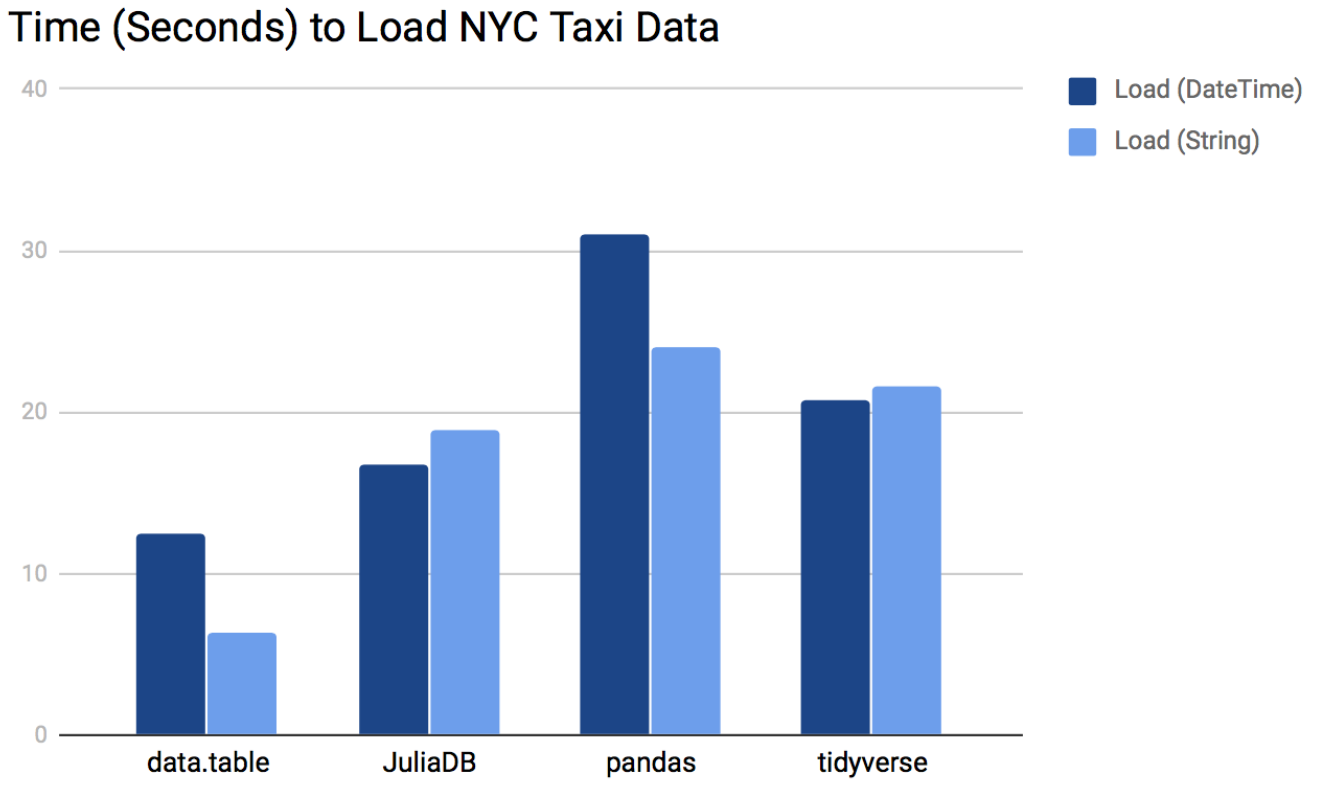
\includegraphics[width=5in]{image8.png} \caption{Performance comparison for loading 815MB from the NYC taxi dataset}
\label{fig:nyctaxiload} 
\end{figure*}
Our test for loading data is an 815 MB CSV file from the NYC Taxi
\& Limousine Commission’s records on every yellow cab trip in January
of 2017. Figure~\ref{fig:nyctaxiload} compares loading times of
this data where the date-time fields are parsed as time objects or
simply as strings.

\subsection{Querying Data}

Our tests for querying involve three different tasks: 
\begin{enumerate}
\item Get the average “fare amount” by type of vendor. This is a standard
“group by” operation, calculating a statistic (mean) grouped by the
unique values in another column (type of vendor). 
\item Get the distribution of “number of passengers” by “day of week”. Here
we wish to count the number of trips where the number of passengers
is one, two, three, etc. grouped by the day of the week. 
\item Get the distribution of “number of passengers” by whether the weekday
number is even (Monday, Wednesday, Friday) or odd (Sunday, Tuesday,
Thursday, Saturday). Here we perform a similar “group by” operation
to the previous task, but use an arbitrary “group by” variable that
needs to depend on a user-defined function. 
\end{enumerate}
JuliaDB is the only platform that does not have a slowdown associated
with a UDF, with pandas taking the biggest hit (Figure~\ref{fig:nyctaxiquery}).

\begin{figure*}[h]
    \centering 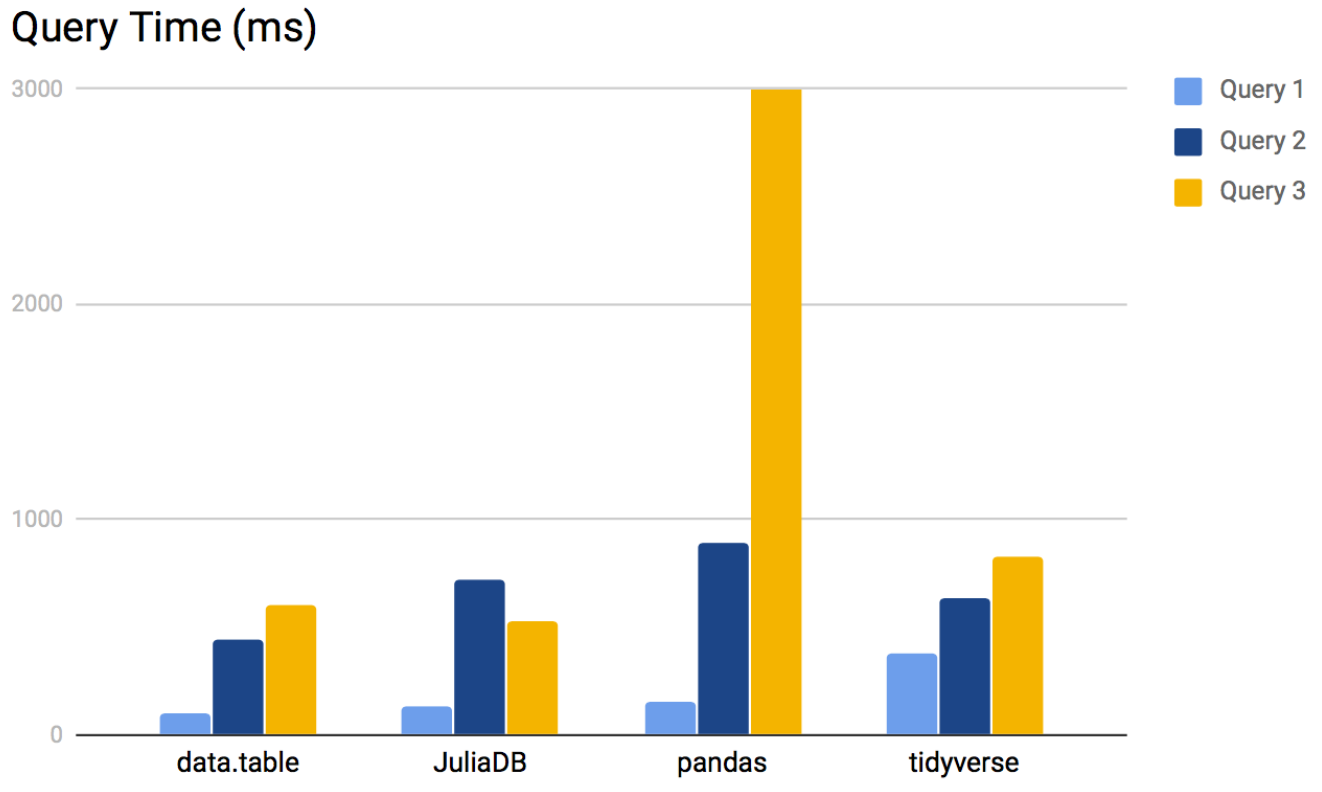
\includegraphics[width=5in]{image4.png}
    \label{fig:nyctaxiquery} 
    \caption{Query performance comparison with other systems. Query 1: average fare amount by type of vendor. Query 2: number of trips grouped by number of passengers and day of week. Query 3: number of trips grouped by number of passengers and even and odd days of week. (Monday, Wednesday, Firday are even, rest are odd).}
\end{figure*}

\section{Usage in real world}

Josh Day describes how JuliaDB is a natural time-series database~\cite{wilmott2018} for large datasets without having been designed with the specific purpose of time-series in mind. JuliaDB is used by the package Diversity.jl~\cite{claireh2018} to generate results in understanding the evolutionary relationships between species across the whole kingdom of flowering plants, and simulations to predict responses of plants species to climate change.

\section{Future directions}

1. AxisArrays
2. Query planning
3. More support for unstructured data

\section{Acknowledgements}

Tanmay Mohapatra, David Anthoff, Jacob Quinn

% **************GENERATED FILE, DO NOT EDIT**************

\bibliographystyle{juliacon}
\bibliography{ref.bib}


\end{document}

% Inspired by the International Journal of Computer Applications template
